% !TeX program = xelatex
\documentclass[UTF8,zihao=-4]{ctexart}

% -------------------- 页面与基础设置 --------------------
\usepackage[a4paper,margin=2.5cm]{geometry}
\linespread{1.25}\selectfont
\setlength{\parindent}{2em}

% -------------------- 数学与排版 --------------------
\usepackage{amsmath,amssymb,amsfonts}
\usepackage{enumitem}
\usepackage{graphicx}
\usepackage{float}
\usepackage[table]{xcolor}
\usepackage{booktabs}
\usepackage{tabularx}
\usepackage{array}
\usepackage{caption}
\usepackage{subcaption}
\usepackage{listings}
\usepackage{fancyhdr}
\usepackage{url}
\usepackage[hidelinks]{hyperref}

% -------------------- 基本信息宏 --------------------
\newcommand{\ReportCourse}{2026 机器学习}
\newcommand{\ReportNo}{2}
\newcommand{\ReportName}{徐厚泽}
\newcommand{\ReportStudentID}{26113050327}

% -------------------- 页眉页脚 --------------------
\pagestyle{fancy}
\fancyhf{}
\fancyfoot[C]{\thepage}
\renewcommand{\headrulewidth}{0pt}

% -------------------- 代码样式 --------------------
\lstdefinestyle{PythonCode}{
  language=Python,
  numbers=left,
  numberstyle=\tiny\color{gray},
  xleftmargin=2.2em,
  basicstyle=\ttfamily\small,
  keywordstyle=\color{blue!70!black}\bfseries,
  stringstyle=\color{green!40!black},
  commentstyle=\color{gray!70!black},
  breaklines=true,
  breakatwhitespace=false,
  columns=flexible,
  frame=single,
  rulecolor=\color{black!20},
  backgroundcolor=\color{black!3}
}
\lstset{style=PythonCode}

% -------------------- 图表与列表样式 --------------------
\captionsetup{font=small,labelfont=bf,labelsep=quad}
\setlist{itemsep=0.25em,topsep=0.25em,parsep=0pt,partopsep=0pt}

% -------------------- 常用自定义命令 --------------------
\newcommand{\mlExperiment}[2]{\subsection{实验#1：#2}}
\newcommand{\mlConclusion}[1]{\par\noindent\textbf{结论#1：}}

\begin{document}

% -------------------- 封面 --------------------
\begin{titlepage}
  \centering
  \vspace*{1.2cm}
  {\heiti\zihao{1}\ReportCourse\par}
  \vspace{1.5em}
  {\heiti\zihao{1}课程报告\ReportNo\par}
  \vfill
  {\kaishu\zihao{-3}姓名：\ReportName\par}
  \vspace{0.8em}
  {\kaishu\zihao{-3}学号：\ReportStudentID\par}
  \vfill
\end{titlepage}

% -------------------- 正文 --------------------
\section{任务描述}
本次作业围绕多层感知机神经网络（Multi-Layer Perceptron Neural Network, MLPNN）的设计与实现展开，包含两个任务：

\textbf{任务一（分类）}：基于 MNIST 手写数字数据集，设计并实现 MLPNN 分类器，完成 10 类手写数字（0--9）的分类任务，并通过对比实验分析网络深度、正则化与训练策略对性能的影响。评价指标为测试集分类准确率（accuracy），并辅以训练损失曲线与混淆矩阵进行分析。

\textbf{任务二（回归）}：基于波士顿房价（Boston House Prices）数据集，设计并实现一个 MLPNN 回归系统，根据 13 个房屋/区域特征预测房价中位数。评价指标为测试集均方误差（MSE）、均方根误差（RMSE）、平均绝对误差（MAE）与决定系数 $R^2$，并与线性回归 baseline 对比；另用 5 折交叉验证评估模型稳定性。

实验环境：NVIDIA A100 (80GB) GPU，PyTorch 2.14.1 (CUDA 13.0)，scikit-learn 1.9.1，Python 3.11。

\section{数据描述}
\subsection{MNIST 数据集}
MNIST 是手写数字识别领域的经典数据集\footnote{下载地址：\url{http://yann.lecun.com/exdb/mnist/}，实验通过 torchvision 自动下载。}，包含 70000 张 $28\times 28$ 的灰度图像，其中训练集 60000 张、测试集 10000 张，每张图像对应 $0\sim 9$ 的一个数字标签，各类别样本数量大致均衡。实验直接使用官方训练/测试划分，不再额外划分验证集。

\subsection{波士顿房价数据集}
波士顿房价数据集\footnote{原始来源：Harrison \& Rubinfeld (1978)，来自 Kaggle（\url{https://www.kaggle.com/vikrishnan/boston-house-prices}）。由于该数据集已在新版 scikit-learn 中移除，本次实验从公开镜像下载原始 CSV（506 行 $\times$ 14 列）。}是回归分析的经典数据集，共 506 个样本，每个样本包含 13 个特征与 1 个回归目标 MEDV（自住房屋价格中位数，单位：千美元，取值范围 5.0--50.0，均值约 22.5）。13 个特征涵盖犯罪率（CRIM）、住宅用地比例（ZN）、非零售商业用地比例（INDUS）、是否紧邻查尔斯河（CHAS）、一氧化氮浓度（NOX）、平均房间数（RM）、老旧房屋比例（AGE）、到就业中心距离（DIS）、公路可达性（RAD）、财产税率（TAX）、师生比（PTRATIO）、族群结构指标（B）与低收入人群比例（LSTAT）。实验将数据按 64\%/16\%/20\% 随机划分为训练集（323 样本）/验证集（80 样本）/测试集（103 样本），随机种子固定为 42 以保证可复现。

\section{数据预处理}
\subsection{MNIST}
预处理包含：(1) 将 PIL 图像转为 float32 张量并把像素值由 $[0,255]$ 缩放到 $[0,1]$；(2) 用 MNIST 统计数据（均值 0.1307、标准差 0.3081）做标准化；(3) 仅改进实验启用随机仿射数据增强（旋转 $\pm10^\circ$、平移 $\pm10\%$、缩放 $[0.9,1.1]$）。MLP 输入时将 $28\times28$ 图像展平为 784 维向量。

\subsection{波士顿房价}
特征之间量纲差异极大（如 TAX 在数百量级、CHAS 为 0/1），直接使用会导致梯度尺度失衡，因此对每个特征做 Z-score 标准化（均值、标准差仅在训练集上计算，避免数据泄漏）；回归目标同样先标准化再训练，评估时还原为原始量纲（千美元）：

\begin{lstlisting}
# 训练集统计量 -> 标准化特征与标签
x_mean, x_std = X[tr].mean(0), X[tr].std(0) + 1e-8
y_mean, y_std = y[tr].mean(0), y[tr].std(0) + 1e-8
Xs = (X - x_mean) / x_std
ys = (y - y_mean) / y_std
\end{lstlisting}

\section{算法介绍}
\subsection{算法原理}
MLPNN 是由若干全连接层堆叠而成的前馈神经网络。设第 $l$ 层输入为 $a^{(l-1)}$，则前向传播为
\[
  z^{(l)} = W^{(l)} a^{(l-1)} + b^{(l)}, \qquad a^{(l)} = \phi\big(z^{(l)}\big),
\]
其中 $\phi$ 为非线性激活函数（本实验默认使用 ReLU）。根据通用近似定理，含足够神经元的单隐层网络即可逼近任意连续函数；增加深度可以提升特征表达能力。网络通过误差反向传播（backpropagation）计算梯度，并用基于 mini-batch 的 Adam 优化器更新参数。两个任务的区别仅在于输出层与损失函数：
\begin{itemize}
  \item \textbf{分类（MNIST）}：输出 10 维 logits，使用交叉熵损失 $\mathcal{L}=-\sum_c y_c\log\hat p_c$（其中 $\hat p = \mathrm{softmax}(z)$）；
  \item \textbf{回归（波士顿房价）}：输出 1 维，使用均方误差损失 $\mathcal{L}=\frac{1}{n}\sum_i(\hat y_i - y_i)^2$。
\end{itemize}
为防止过拟合，实验用到以下正则化技术：(1) \textbf{Dropout}：训练时以概率 $p$ 随机丢弃神经元；(2) \textbf{权重衰减}（$L_2$ 正则）；(3) \textbf{早停（early stopping）}：回归任务中以验证集 RMSE 为准，连续若干轮不下降即停止并恢复最优权重；(4) \textbf{数据增强}与余弦退火学习率（仅 MNIST 改进实验）。

\subsection{算法实现}
实现一个通用 MLP 类同时服务两个任务：输入维度、隐藏层列表、输出维度、激活函数、Dropout 与 BatchNorm 均可配置。核心代码如下：

\begin{lstlisting}
class MLP(nn.Module):
    """Input -> [Linear -> (BN) -> Act -> (Dropout)] x L -> Linear(out)"""
    def __init__(self, input_dim, hidden_sizes, output_dim,
                 activation="relu", dropout=0.0, use_bn=False):
        super().__init__()
        layers, d_in = [], input_dim
        for d in hidden_sizes:
            layers += [nn.Linear(d_in, d), ACTS[activation]()]
            if dropout > 0:
                layers.append(nn.Dropout(dropout))
            d_in = d
        layers.append(nn.Linear(d_in, output_dim))
        self.net = nn.Sequential(*layers)

    def forward(self, x):
        if x.dim() > 2:            # 图像输入时展平
            x = x.view(x.size(0), -1)
        return self.net(x)
\end{lstlisting}

分类任务训练流程与作业1一致：批大小 128，Adam（初始学习率 $10^{-3}$），训练 15 epoch，每个 epoch 在完整测试集上评估。回归任务由于数据量小（训练集仅 323 个样本），采用小批量（32）全数据迭代、最多 500 epoch、早停耐心 60，模型选择以验证集 RMSE 最优的 epoch 为准；此外实现了 5 折交叉验证用于稳健评估，并以 scikit-learn 的线性回归作为 baseline。

\section{实验结果及分析}

\mlExperiment{5.1}{MNIST 分类：Baseline MLP 与改进实验}
Baseline 为单隐层 MLP（784--256--10），批大小 128，Adam 学习率 $10^{-3}$，训练 15 epoch，训练集 60000 张、测试集 10000 张。在此基础上采用逐项累加的消融设计：加深网络（双隐层 512--256）$\to$ 加入 Dropout(0.3) 与权重衰减（$5\times10^{-4}$）$\to$ 再加入数据增强与余弦退火学习率。结果见表~\ref{tab:mnist} 与图~\ref{fig:mnist_curves}、图~\ref{fig:mnist_cm}。

\begin{table}[H]
  \centering
  \caption{MNIST 各实验结果对比（训练 15 epoch）}
  \label{tab:mnist}
  \begin{tabular}{lcccc}
    \toprule
    实验 & 参数量 & 最优测试准确率/\% & 最终测试准确率/\% & 训练时间/s \\
    \midrule
    MLP 784--256--10（baseline） & 203,530 & 98.15 & 98.02 & 47.9 \\
    MLP 784--512--256--10 & 535,818 & 98.38 & 98.38 & 47.6 \\
    + Dropout \& 权重衰减 & 535,818 & 98.04 & 97.96 & 47.2 \\
    + 数据增强 \& 余弦学习率 & 535,818 & \textbf{98.90} & \textbf{98.90} & 114.1 \\
    \bottomrule
  \end{tabular}
\end{table}

\begin{figure}[H]
  \centering
  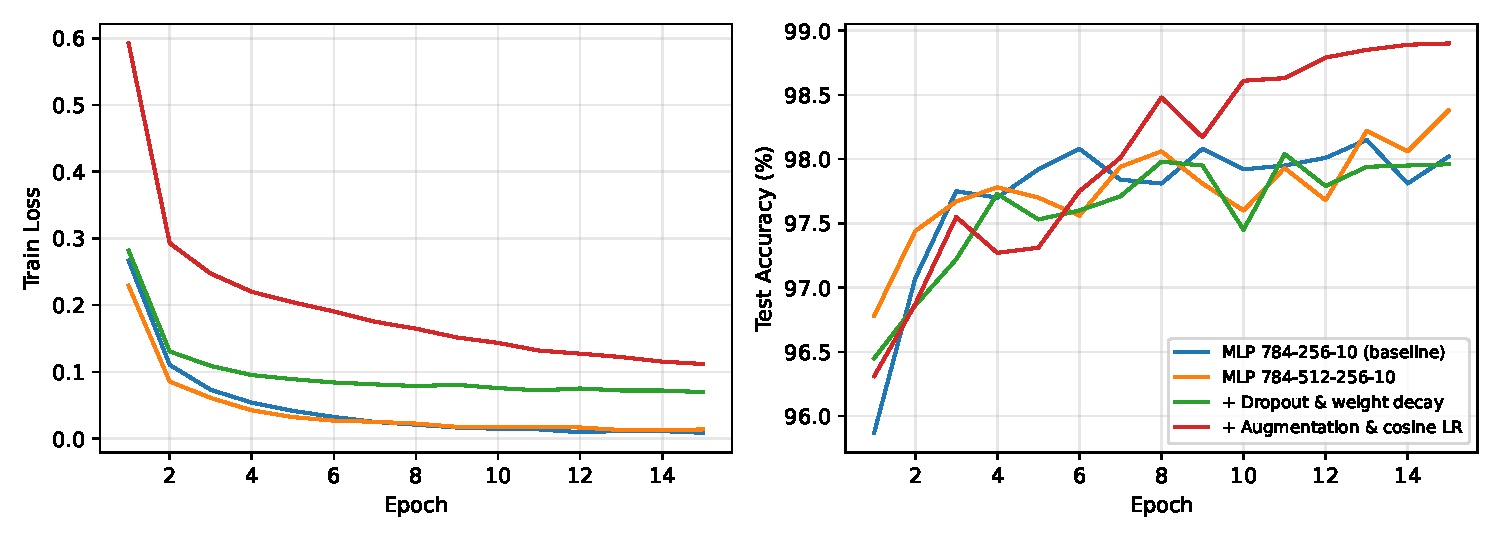
\includegraphics[width=\textwidth]{figures/mnist_training_curves.pdf}
  \caption{MNIST 各实验训练损失（左）与测试准确率（右）曲线}
  \label{fig:mnist_curves}
\end{figure}

\begin{figure}[H]
  \centering
  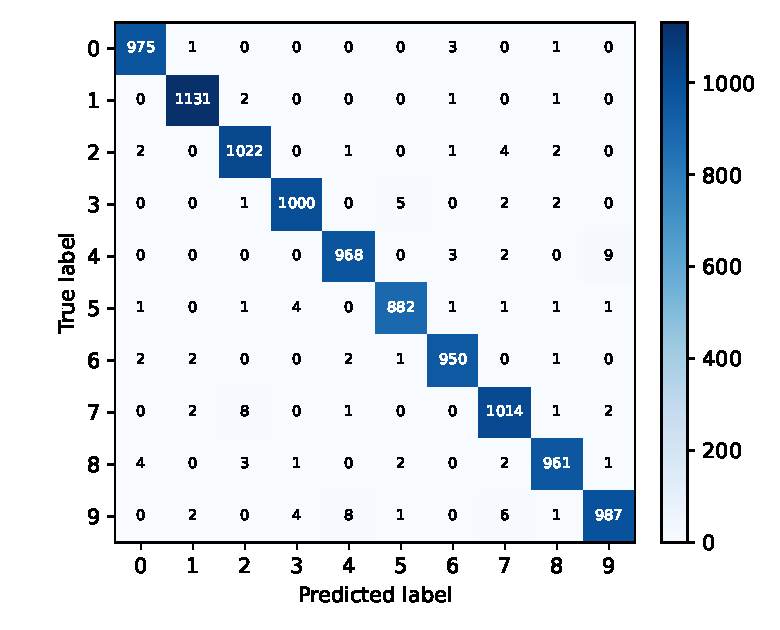
\includegraphics[width=0.62\textwidth]{figures/mnist_confusion_matrix.pdf}
  \caption{完整改进 MLP 的测试集混淆矩阵（110/10000 个样本分类错误）}
  \label{fig:mnist_cm}
\end{figure}

\mlConclusion{1}
结果分析如下：
\begin{enumerate}
  \item 单隐层 MLP 即可在 MNIST 上达到 98.15\% 的准确率，验证了 MLP 对简单图像分类任务的有效性；加深为双隐层（512--256）后提升至 98.38\%，体现了深度带来的表达能力提升；
  \item 单独加入 Dropout 与权重衰减反而使最优准确率略降至 98.04\%，说明在 MNIST 这类简单任务上 MLP 的容量并未过剩，较强的正则化带来轻微欠拟合；
  \item 加入随机仿射数据增强与余弦退火学习率后，测试准确率随训练进行持续上升并最终达到 98.90\%，训练与测试曲线几乎贴合，说明等效的"数据扩容"+平滑学习率衰减显著提升了泛化能力，此时正则化的作用才真正发挥出来；
  \item 混淆矩阵（图~\ref{fig:mnist_cm}）显示错误共 110 个，主要集中在易混数字对 4$\leftrightarrow$9（17 次）、7$\to$2（8 次）、9$\to$7（6 次）、3$\leftrightarrow$5（9 次）。与作业1的 CNN（99.66\%）相比仍有约 0.8 个百分点的差距，说明 MLP 对图像空间结构的建模能力弱于卷积结构，但对于课程要求的"MLPNN 分类器"而言该性能已属正常水平。
\end{enumerate}

\mlExperiment{5.2}{波士顿房价回归：MLPNN 回归系统}
Baseline 为 scikit-learn 线性回归；MLP 采用 13--32--1（无正则）与 13--64--32--1（Dropout 0.1 + 权重衰减 $10^{-4}$ + 早停）两种配置，Adam 学习率 $10^{-3}$、批大小 32、最多 500 epoch。结果见表~\ref{tab:boston} 与图~\ref{fig:boston_curves}、图~\ref{fig:boston_scatter}。

\begin{table}[H]
  \centering
  \caption{波士顿房价各实验结果对比（同一切分：train/val/test = 323/80/103）}
  \label{tab:boston}
  \begin{tabular}{lccccc}
    \toprule
    实验 & 参数量 & 测试 RMSE（千美元）$\downarrow$ & 测试 MAE（千美元）$\downarrow$ & 测试 $R^2\uparrow$ \\
    \midrule
    线性回归（baseline） & 14 & 4.732 & 3.194 & 0.6824 \\
    MLP 13--32--1（无正则） & 481 & 3.493 & 2.417 & 0.8270 \\
    MLP 13--64--32--1 + Dropout + 权重衰减 & 3,009 & \textbf{2.922} & \textbf{2.054} & \textbf{0.8789} \\
    \midrule
    MLP 13--64--32--1，5 折交叉验证 & 3,009 & \multicolumn{2}{c}{$3.191\pm0.339$} & $0.8744\pm0.0301$ \\
    \bottomrule
  \end{tabular}
\end{table}

\begin{figure}[H]
  \centering
  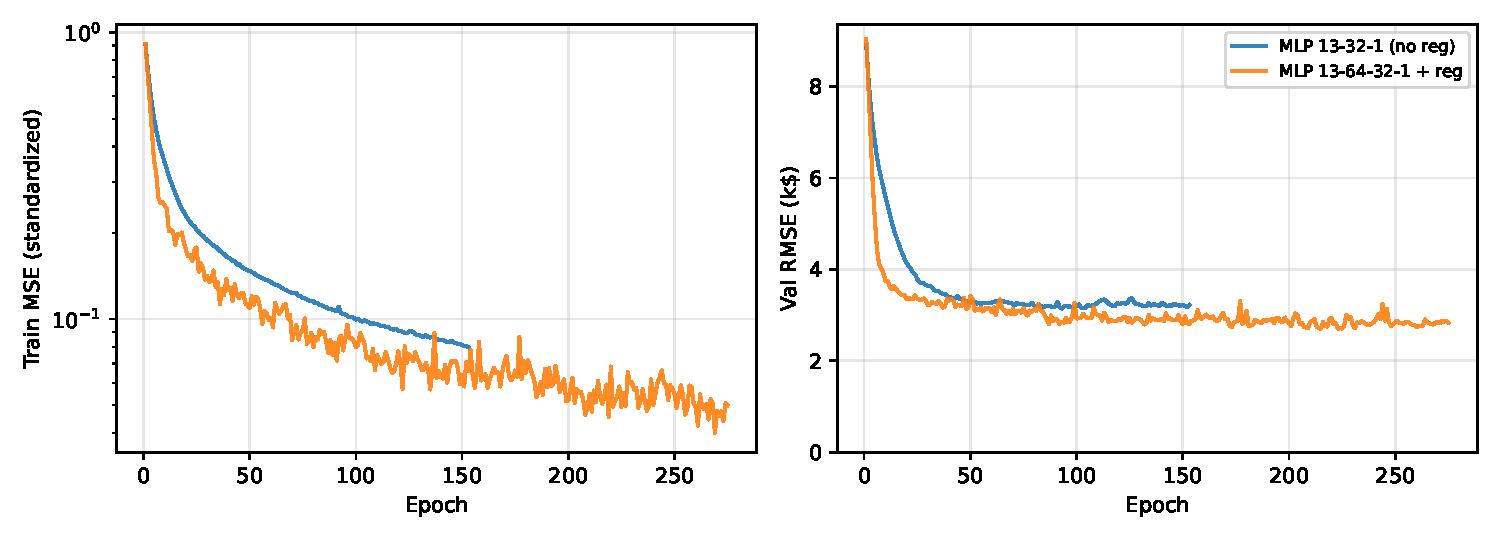
\includegraphics[width=\textwidth]{figures/boston_training_curves.pdf}
  \caption{房价回归训练 MSE（左，标准化量纲，对数轴）与验证集 RMSE（右，千美元）曲线}
  \label{fig:boston_curves}
\end{figure}

\begin{figure}[H]
  \centering
  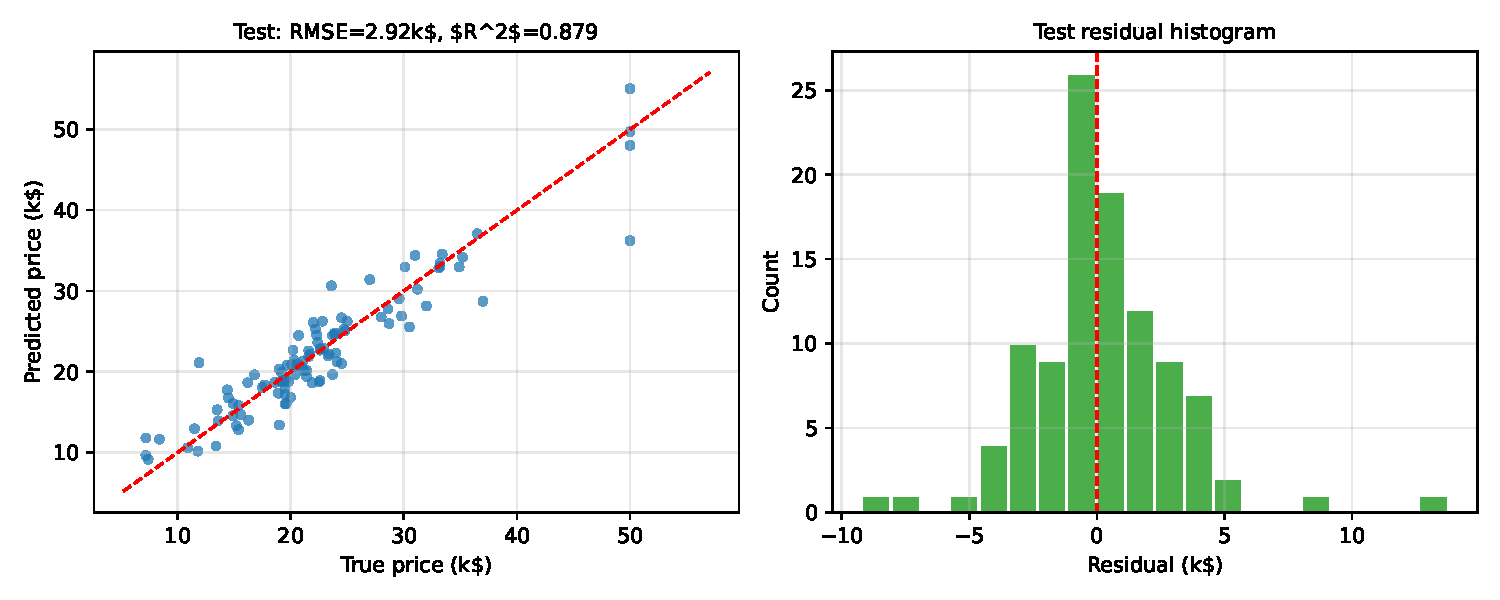
\includegraphics[width=\textwidth]{figures/boston_pred_vs_true.pdf}
  \caption{最优 MLP 在测试集上的预测值--真实值散点图（左）与残差直方图（右）}
  \label{fig:boston_scatter}
\end{figure}

\mlConclusion{2}
结果分析如下：
\begin{enumerate}
  \item 线性回归仅取得 $R^2=0.68$，说明房价与各特征之间存在显著非线性关系；简单的单隐层 MLP 即将 RMSE 由 4.73 降至 3.49（$R^2=0.83$），验证了 MLP 的非线性拟合能力；
  \item 加深加宽并加入 Dropout、权重衰减与早停后，测试 RMSE 进一步降至 2.92 千美元、$R^2=0.879$；由图~\ref{fig:boston_curves} 可见无正则的小网络在约 90 epoch 后验证误差不再下降，而带正则的网络能稳定训练到 215 epoch 才触发早停，泛化能力更强；
  \item 5 折交叉验证给出 RMSE $=3.19\pm0.34$、$R^2=0.874\pm0.030$，与单次划分的结果一致且波动较小，说明模型对该小数据集的划分不算敏感，结论稳健；
  \item 由图~\ref{fig:boston_scatter} 可见预测点整体紧贴对角线，残差近似以 0 为中心对称分布，但在高价区（MEDV 接近 50）出现系统性低估——数据集中房价被人为截断在 50 千美元，这部分样本的真实价格分布未知，是回归误差的主要来源之一。
\end{enumerate}

\section{总结}
本次作业完整设计并实现了通用的 MLPNN 框架，并分别在 MNIST 分类与波士顿房价回归两个任务上完成训练、评估与消融分析。主要结论：(1) 分类任务中，单隐层 MLP 可达 98.15\% 准确率，加深网络、数据增强与余弦学习率可使最佳模型达到 98.90\%，但弱于作业1的 CNN（99.66\%），说明网络结构应匹配数据的空间特性；(2) 回归任务中，MLP 显著优于线性回归（测试 RMSE 由 4.73 降至 2.92 千美元，$R^2$ 由 0.68 提升至 0.88），特征与标签的标准化、Dropout、权重衰减与早停是小样本回归任务上稳定训练的关键；(3) 5 折交叉验证（RMSE $3.19\pm0.34$）确认了回归结果的稳健性。后续可以在回归任务上尝试更适合小表格数据的集成树模型作为对照，在分类任务上尝试更深的 MLP 结合 BN 与残差连接，进一步缩小与卷积网络的差距。

\end{document}
